% ============================================================
% Cheat sheet, argomento 5: dal codice al diagramma, array e collezioni
% ============================================================
\argomento{Dal codice al diagramma: array e collezioni}{Dispensa: capitolo 7. Le collezioni diventano
molteplicità}[Dal codice: array e collezioni]

\begin{guida}{Array e collezioni in un colpo d'occhio}
Se gli elementi sono oggetti di una \textbf{classe del diagramma}, la collezione è un'\textbf{associazione} e la
molteplicità si scrive vicino a quella classe. Se sono valori (\code{int}, \code{String}, \code{LocalDate}\ldots) è
un \textbf{attributo}, con la molteplicità fra quadre: \code{voti: int [*] \{ordered, nonunique\}}.

\centering
\renewcommand{\arraystretch}{1.3}
\begin{tabular}{@{}l l l@{}}
  \textbf{Nel codice} & \textbf{Molteplicità e proprietà} & \textbf{Caso} \\ \hline
  \code{B[] x = new B[n]} & \code{n} se è sempre pieno, \code{0..n} se no; \code{\{ordered\}} & \vv{arrayoggetti} \\
  \code{B[] x} di lunghezza decisa a runtime & \code{*} \code{\{ordered\}} & \vv{arrayoggetti} \\
  \code{int[] x = new int[n]}, \code{String[] x} & attributo \code{x: int [n]}, \code{x: String [*]}, \code{\{ordered\}} & \vv{arrayprimitivi} \\
  \code{List<B>}, \code{ArrayList<B>}, \code{LinkedList<B>} & \code{*} \code{\{ordered\}}, più \code{\{nonunique\}} se ammette doppioni & \vv{lista} \\
  \code{Set<B>}, \code{HashSet<B>} & \code{*} e basta: è il significato predefinito & \vv{insieme} \\
  \code{TreeSet<B>}, \code{LinkedHashSet<B>}, \code{SortedSet<B>} & \code{*} \code{\{ordered\}} & \vv{insieme} \\
  \code{Queue<B>}, \code{Deque<B>}, \code{Stack<B>} & \code{*} \code{\{ordered\}} \oltre & \vv{coda} \\
  \code{Collection<B>}, \code{Iterable<B>} & \code{*} & \vv{coda} \\
  \code{Map<K, B>} & qualificatore \code{k: K}, poi \code{0..1} \oltre & \vv{mappa} \\
  \code{Map<K, List<B>>} & qualificatore \code{k: K}, poi \code{*} \code{\{ordered\}} \oltre & \vv{mappalista} \\
  \code{Optional<B>} & \code{0..1} \oltre & \vv{opzionale} \\
  \code{B[][]} & qualificatori \code{i: int, j: int}, poi \code{0..1} \oltre & \vv{matrice} \\
  almeno uno, al più $n$ (costruttore, controlli) & \code{1..*}, \code{0..n}, \code{1..n} & \vv{vincoli} \\
\end{tabular}

\raggedright La classe concreta (\code{ArrayList}, \code{HashMap}\ldots) \textbf{non} compare nel diagramma: è un
dettaglio di implementazione. E \code{final} su una collezione \textbf{non} è \code{\{readOnly\}}: il riferimento
non cambia, ma gli elementi sì.
\end{guida}

\begin{caso}{arrayoggetti}{Array di oggetti}
\begin{lstlisting}[style=javacs]
class Partita {
    private final Giocatore[] giocatori =
            new Giocatore[2];
    Partita(Giocatore a, Giocatore b) {
        giocatori[0] = a;     // sempre pieno
        giocatori[1] = b;
    }
}
class Squadra {
    private final Giocatore[] rosa =
            new Giocatore[25];
    private int iscritti = 0;
    void iscrivi(Giocatore g) {
        rosa[iscritti++] = g;   // man mano
    }
}
class Torneo {
    private final Squadra[] squadre;
    Torneo(int n) { squadre = new Squadra[n]; }
}
class Giocatore { }
\end{lstlisting}
\tcblower
\begin{tikzpicture}
  \node[classe1=1.6cm] (pa) at (0,0) {Partita};
  \node[classe1=1.8cm] (gi) at (5.2,0) {Giocatore};
  \node[classe1=1.6cm] (sq) at (5.2,-2.1) {Squadra};
  \node[classe1=1.6cm] (to) at (0,-2.1) {Torneo};
  \draw[navig] (pa.east) -- (gi.west);
  \estO{(gi.west)}{2 \{ordered\}}{giocatori}
  \draw[navig] (sq.north) -- (gi.south);
  \estS{(gi.south)}{0..25 \{ordered\}}{rosa}
  \draw[navig] (to.east) -- (sq.west);
  \estO{(sq.west)}{* \{ordered\}}{squadre}
\end{tikzpicture}
\regola{Un array di oggetti è un'associazione, e la molteplicità è la \textbf{lunghezza}: \code{2} se le celle sono
sempre tutte piene, \code{0..25} se si riempiono man mano (le altre restano \code{null}), \code{*} se la lunghezza si
decide durante l'esecuzione. \code{\{ordered\}}: ogni elemento ha un indice.}
\end{caso}

\begin{caso}{arrayprimitivi}{Array di valori: primitivi e String}
\begin{lstlisting}[style=javacs]
class Studente {
    private int[] voti = new int[30];
    private String[] telefoni;
    private char[] codiceFiscale = new char[16];
}
\end{lstlisting}
\tcblower
\begin{tikzpicture}
  \umlclass[6.6cm]{s}{(0,0)}{Studente}{- voti: int [30] \{ordered, nonunique\}\\- telefoni: String [*] \{ordered\}\\- codiceFiscale: char [16] \{ordered, nonunique\}}{}
\end{tikzpicture}
\regola{Un array di valori è un \textbf{attributo} con la molteplicità fra quadre: la lunghezza se è fissa
(\code{[30]}), \code{[*]} se non si conosce. \code{\{ordered\}} perché le celle hanno un indice; \code{\{nonunique\}}
perché lo stesso voto, o la stessa lettera, può ripetersi. Il tipo Java (\code{voti: int[]}) si capisce, ma non è la
notazione UML.}
\end{caso}

\begin{caso}{lista}{Liste di oggetti: List, ArrayList, LinkedList}
\begin{lstlisting}[style=javacs]
class Playlist {
    private String nome;
    private final List<Brano> brani =
            new ArrayList<>();

    void aggiungi(Brano b) { brani.add(b); }
    void rimuovi(Brano b) { brani.remove(b); }
}
class Brano {
    private String titolo;
}
\end{lstlisting}
\tcblower
\begin{tikzpicture}
  \umlclass[3.0cm]{p}{(0,0)}{Playlist}{- nome: String}{+ aggiungi(b: Brano)\\+ rimuovi(b: Brano)}
  \umlclass[2.2cm]{b}{(5.8,0)}{Brano}{- titolo: String}{}
  \draw[navig] (p.east |- b.west) -- (b.west);
  \estO{(b.west)}{* \{ordered, nonunique\}}{brani}
\end{tikzpicture}
\regola{\code{List}, \code{ArrayList}, \code{LinkedList}, \code{Vector}: associazione \code{*} \code{\{ordered\}}; il
nome della lista è il ruolo. Qui anche \code{\{nonunique\}}, perché lo stesso brano può comparire due volte; in una
lista dove ogni oggetto c'è una volta sola basta \code{\{ordered\}}. Con \code{new ArrayList} o \code{new
LinkedList} il diagramma non cambia.}
\end{caso}

\begin{caso}{listavalori}{Liste di valori}
\begin{lstlisting}[style=javacs]
class Ricetta {
    private final List<String> ingredienti =
            new ArrayList<>();
    private final List<Integer> tempi =
            new LinkedList<>();
}
\end{lstlisting}
\tcblower
\begin{tikzpicture}
  \umlclass[6.0cm]{r}{(0,0)}{Ricetta}{- ingredienti: String [*] \{ordered\}\\- tempi: Integer [*] \{ordered, nonunique\}}{}
\end{tikzpicture}
\regola{Una collezione di \code{String}, \code{Integer} o altri tipi di libreria è un \textbf{attributo} con
molteplicità, non un'associazione (non c'è una classe \code{String} nel diagramma). \code{final} non diventa
\code{\{readOnly\}}: la lista è sempre la stessa, ma il suo contenuto cambia.}
\end{caso}

\begin{caso}{insieme}{Insiemi: Set, HashSet, TreeSet, LinkedHashSet}
\begin{lstlisting}[style=javacs]
class Corso {
    private final Set<Studente> iscritti =
            new HashSet<>();
    private final Set<Studente> perArrivo =
            new LinkedHashSet<>(); // per arrivo
    private final Set<String> aule =
            new TreeSet<>();       // alfabetico
}
class Studente { }
\end{lstlisting}
\tcblower
\begin{tikzpicture}
  \umlclass[3.6cm]{c}{(0,0)}{Corso}{- aule: String [*] \{ordered\}}{}
  \node[classe1=1.8cm, minimum height=1.0cm] (s) at (5.6,0) {Studente};
  \draw[navig] ($(c.east)+(0,0.25)$) -- ($(s.west)+(0,0.25)$);
  \draw[navig] ($(c.east)+(0,-0.25)$) -- ($(s.west)+(0,-0.25)$);
  \node[ruolo, anchor=south east] at ($(s.west)+(-0.1,0.32)$) {iscritti};
  \node[molt, anchor=north east] at ($(s.west)+(-0.1,0.18)$) {*};
  \node[molt, anchor=south east] at ($(s.west)+(-0.1,-0.18)$) {* \{ordered\}};
  \node[ruolo, anchor=north east] at ($(s.west)+(-0.1,-0.32)$) {perArrivo};
\end{tikzpicture}
\regola{\code{Set} e \code{HashSet}: \code{*} senza proprietà, perché per UML una molteplicità è già un insieme
(niente doppioni, niente ordine). \code{LinkedHashSet} (ordine di inserimento) e \code{TreeSet} (ordine naturale):
\code{\{ordered\}}. In un insieme i doppioni non ci sono mai, quindi mai \code{\{nonunique\}}.}
\end{caso}

\begin{caso}{coda}{Code, pile e collezioni generiche \oltre}
\begin{lstlisting}[style=javacs]
class Sportello {
    private final Queue<Cliente> inAttesa =
            new ArrayDeque<>();  // coda: FIFO
    private final Deque<Pratica> daFirmare =
            new ArrayDeque<>();  // pila: LIFO
    private final Collection<Cliente> serviti =
            new ArrayList<>();
}
class Cliente { }
class Pratica { }
\end{lstlisting}
\tcblower
\begin{tikzpicture}
  \node[classe1=1.8cm, minimum height=1.0cm] (s) at (0,0) {Sportello};
  \node[classe1=1.6cm, minimum height=1.0cm] (c) at (5.6,0) {Cliente};
  \node[classe1=1.6cm] (p) at (5.6,-1.6) {Pratica};
  \draw[navig] ($(s.east)+(0,0.25)$) -- ($(c.west)+(0,0.25)$);
  \draw[navig] ($(s.east)+(0,-0.25)$) -- ($(c.west)+(0,-0.25)$);
  \node[ruolo, anchor=south east] at ($(c.west)+(-0.1,0.32)$) {inAttesa};
  \node[molt, anchor=north east] at ($(c.west)+(-0.1,0.18)$) {* \{ordered\}};
  \node[molt, anchor=south east] at ($(c.west)+(-0.1,-0.18)$) {*};
  \node[ruolo, anchor=north east] at ($(c.west)+(-0.1,-0.32)$) {serviti};
  \draw[navig] (s.south) |- (p.west);
  \estO{(p.west)}{* \{ordered\}}{daFirmare}
\end{tikzpicture}
\regola{\code{Queue}, \code{Deque}, \code{Stack}: \code{*} \code{\{ordered\}}, perché chi esce dipende dall'ordine
(FIFO o LIFO: lo si può scrivere in una nota). \code{Collection} e \code{Iterable} non promettono né ordine né
unicità: \code{*} e basta.}
\end{caso}

\begin{caso}{mappa}{Mappe da una chiave a un oggetto \oltre}
\begin{lstlisting}[style=javacs]
class Rubrica {
    private final Map<String, Contatto> perNome =
            new HashMap<>();
    void aggiungi(String nome, Contatto c) {
        perNome.put(nome, c);
    }
    Contatto cerca(String nome) {
        return perNome.get(nome);
    }
}
class Contatto {
    private String telefono;
}
\end{lstlisting}
\tcblower
\begin{tikzpicture}
  \node[classe1=1.6cm] (r) at (0,0) {Rubrica};
  \node[draw=black!80, fill=white, line width=0.7pt, font=\tiny, inner sep=2pt, minimum height=0.55cm,
        anchor=west] (q) at (r.east) {nome: String};
  \umlclass[2.4cm]{c}{(5.6,-0.12)}{Contatto}{- telefono: String}{}
  \draw[navig] (q.east) -- (q.east -| c.west);
  \estO{(q.east -| c.west)}{0..1}{perNome}
\end{tikzpicture}
\regola{\code{Map<K, V>} con \code{V} classe del diagramma: \textbf{associazione qualificata}. Il qualificatore è la
chiave (\code{nome: String}); \code{0..1} vale \textbf{per ogni chiave}: dato un nome, al più un contatto. Se il
qualificatore non serve, va bene anche un'associazione \code{*} con il ruolo \code{perNome}.}
\end{caso}

\begin{caso}{mappalista}{Mappe da una chiave a una lista \oltre}
\begin{lstlisting}[style=javacs]
class Biblioteca {
    private final Map<String, List<Libro>>
            perAutore = new HashMap<>();
    List<Libro> diAutore(String autore) {
        return perAutore.getOrDefault(autore,
                                      List.of());
    }
}
class Libro {
    private String titolo;
}
\end{lstlisting}
\tcblower
\begin{tikzpicture}
  \node[classe1=1.8cm] (b) at (0,0) {Biblioteca};
  \node[draw=black!80, fill=white, line width=0.7pt, font=\tiny, inner sep=2pt, minimum height=0.55cm,
        anchor=west] (q) at (b.east) {autore: String};
  \umlclass[2.2cm]{l}{(6.0,-0.12)}{Libro}{- titolo: String}{}
  \draw[navig] (q.east) -- (q.east -| l.west);
  \estO{(q.east -| l.west)}{* \{ordered\}}{perAutore}
\end{tikzpicture}
\regola{La chiave seleziona un \textbf{gruppo}: dopo il qualificatore la molteplicità è quella della lista,
\code{*} \code{\{ordered\}}. Con \code{Map<String, Set<Libro>>} sarebbe \code{*} senza proprietà.}
\end{caso}

\begin{caso}{mappavalori}{Mappe di valori \oltre}
\begin{lstlisting}[style=javacs]
class Magazzino {
    private final Map<String, Integer> giacenze =
            new HashMap<>();
    int quantita(String codice) {
        return giacenze.getOrDefault(codice, 0);
    }
}
\end{lstlisting}
\tcblower
\begin{tikzpicture}
  \umlclass[5.6cm]{m}{(0,0)}{Magazzino}{- giacenze: Map<String, Integer>}{+ quantita(codice: String): int}
\end{tikzpicture}
\regola{Se chiave e valore sono tipi di libreria, la mappa è un \textbf{attributo} con il suo tipo Java. Se la coppia
ha un significato nel dominio, è meglio una classe (\code{Giacenza}, con \code{codice} e \code{quantita}) e
un'associazione \code{*} verso di lei.}
\end{caso}

\begin{caso}{opzionale}{Optional \oltre}
\begin{lstlisting}[style=javacs]
class Utente {
    private Indirizzo indirizzo;   // può mancare
    Optional<Indirizzo> getIndirizzo() {
        return Optional.ofNullable(indirizzo);
    }
}
class Indirizzo {
    private String via;
}
\end{lstlisting}
\tcblower
\begin{tikzpicture}
  \umlclass[4.4cm]{u}{(0,0)}{Utente}{}{+ getIndirizzo(): Indirizzo [0..1]}
  \umlclass[2.2cm]{i}{(5.0,-1.7)}{Indirizzo}{- via: String}{}
  \draw[navig] (u.south) |- (i.west);
  \estO{(i.west)}{0..1}{indirizzo}
\end{tikzpicture}
\regola{\code{Optional<T>} vuol dire «zero o uno»: \code{0..1}. Come tipo di ritorno si scrive \code{T [0..1]}; come
campo, \code{Optional<Indirizzo>} si disegna come un \code{Indirizzo} che può essere \code{null}, cioè
un'associazione \code{0..1}.}
\end{caso}

\begin{caso}{matrice}{Matrici \oltre}
\begin{lstlisting}[style=javacs]
class Scacchiera {
    private final Casella[][] caselle =
            new Casella[8][8];
    Casella casella(int riga, int colonna) {
        return caselle[riga][colonna];
    }
}
class Casella { }

class Immagine {
    private int[][] pixel = new int[600][800];
}
\end{lstlisting}
\tcblower
\begin{tikzpicture}
  \node[classe1=1.9cm] (s) at (0,0) {Scacchiera};
  \node[draw=black!80, fill=white, line width=0.7pt, font=\tiny, inner sep=2pt, minimum height=0.55cm, align=left,
        anchor=west] (q) at (s.east) {riga: int\\colonna: int};
  \node[classe1=1.6cm] (c) at (5.8,0) {Casella};
  \draw[navig] (q.east) -- (c.west);
  \estO{(c.west)}{0..1}{caselle}
  \umlclass[5.0cm]{im}{(2.5,-1.6)}{Immagine}{- pixel: int[][] \{600 $\times$ 800\}}{}
\end{tikzpicture}
\regola{UML non ha molteplicità a due dimensioni. Per una matrice di \textbf{oggetti} si usa un'associazione
qualificata con \textbf{due} qualificatori: data riga e colonna, al più una casella (\code{1} se è sempre piena). Per
una matrice di \textbf{valori} si scrive il tipo Java, con le dimensioni in una nota o fra graffe; in alternativa
la riga diventa una classe.}
\end{caso}

\begin{caso}{vincoli}{Almeno uno, al più quattro: i vincoli del codice}
\begin{lstlisting}[style=javacs]
class Squadra {
    private static final int MAX = 4;
    private final List<Giocatore> giocatori =
            new ArrayList<>();

    Squadra(Giocatore capitano) {   // almeno uno
        giocatori.add(capitano);
    }
    void aggiungi(Giocatore g) {   // al più 4
        if (giocatori.size() == MAX)
            throw new IllegalStateException();
        giocatori.add(g);
    }
}
class Giocatore { }
\end{lstlisting}
\tcblower
\begin{tikzpicture}
  \umlclass[3.8cm]{s}{(0,0)}{Squadra}{\underline{- MAX: int = 4 \{readOnly\}}}{\textasciitilde\ aggiungi(g: Giocatore)}
  \node[classe1=1.8cm] (g) at (5.8,0) {Giocatore};
  \draw[navig] (s.east |- g.west) -- (g.west);
  \estO{(g.west)}{1..4 \{ordered\}}{giocatori}
\end{tikzpicture}
\regola{La molteplicità viene da ciò che il codice \textbf{garantisce}: il costruttore mette subito un giocatore
(minimo \code{1}), il controllo in \code{aggiungi} impedisce il quinto (massimo \code{4}). Nel testo
dell'esercizio la stessa informazione è «squadre di al più 4 giocatori, con un capitano».}
\end{caso}
